\documentclass[fr]{../../../eplsummary}

\usepackage{gensymb}

\hypertitle{Méthodes et conceptions géotechniques}{8}{GCIV}{2072}
{Thomas Wyckmans}
{Alain Holeyman}

\part{Reconnaissance géotechnique in situ}

\section{Introduction}

La reconnaissance géotechnique a pour but de :
\begin{itemize}
    \item Définir l'état et les caractéristiques des formations rencontrées sur le site.
    \item Prévoir les difficultés qui pourront être rencontrées durant la restauration ou l'exécution du projet dû au terrain.
    \item Proposer les solutions correspondantes ou à défaut, les études plus détaillées nécessaires.
\end{itemize}

\subsection{Essais in situ}

\begin{center}
    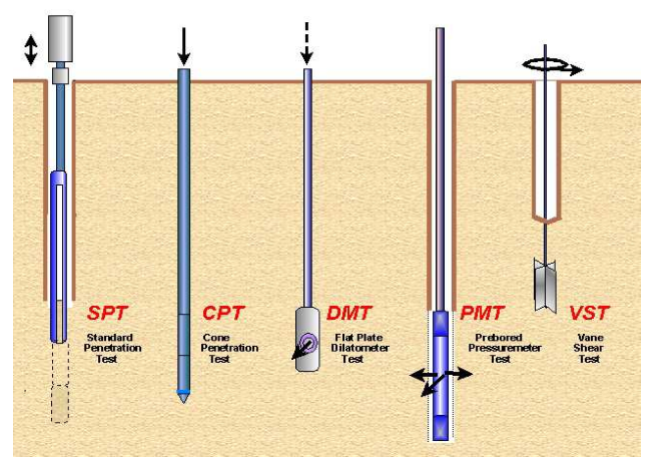
\includegraphics[scale=1]{images/photo1.PNG}
\end{center}

\begin{itemize}
    \item Cone penetration test (CPT)
    \item Standard penetration test (SPT)
    \item Cone penetration test with pore water pressure data (CPTu)
    \item Dilatometer tes (DMT)
    \item pressiomètre (PMT)
\end{itemize}

\subsection{Ampleur et densité de reconnaissance}

Un nombre trop faible de forages ne peu pas caractériser efficacement toute la surface, on aura un manque de résolution. A l'inverse un nombre trop élevé se traduit par un coût et un temps de réalisation considérable (trop de forage risque de détériorer le sol par liquéfaction). Il faut trouver un juste milieu en fonction de:

\begin{itemize}
    \item Du type et de la taille du projet
    \item Du contexte géotechnique 
    \item Du budget
\end{itemize}

Il faut pas combiner les essais de surface (sismique) avec des essais de pénétration.

\underline{Disposition des points de reconnaissance :}

\begin{itemize}
    \item On ne dépasse pas 25-30m entre les essais.
    \item Les situer sur des charges anticipées
    \item Se positionner aux extrémités
    \item aligner les essais pour faciliter l'établissement de coupes
\end{itemize} 

\underline{Profondeur de reconnaissance :} 

La profondeur correspond généralement à la dimension verticale du bulbe d'influence (environ deux fois la taille de la fondation); ou plus précisément, jusqu'à ce que la variation des contraintes devienne négligeable. Il faut prendre en compte le terrassement !

\section{Essai de pénétration standard (SPT)}

\subsection{Déroulement de l'essai}

On combine un essai de prélèvement avec un essai dynamique. Il ne faut pas être trop exigeant avec les résultats, la plupart étant basées sur une approche pragmatique et empirique.

\begin{itemize}
    \item On réalise un forage et on introduit un carottier.
    \item On l'enfonce par battage avec un mouton (SPT) en mesurant le nombre de coups nécessaire (3 volées de coups pour un enfoncement de 15cm chacun) (mouton = 65kg et hauteur = 76cm).
    \item On obtient l'indice de pénétration (N-value) soit le nombre de coups nécessaire pour enfoncer le carottier d'un pied, soit la somme des deux dernières volées.
\end{itemize} 

\subsection{Utilisation des résultats}

Fiable pour des sols pulvérulents (sable). On obtient des échantillons fortement remaniés (si le sol le permet on préfère un carottier plus mince pour moins de remaniement). 
Il s'agit d'un essai discontinu réalisé à intervalle de 1.5m. Il est facile à réaliser, peu technologique, rapide et économique.

\subsection{Normalisation de l'indice de pénétration}

On apporte quelques modifications :

\begin{center}
\begin{tabular}{c|c}
    $(N_1)_{60} = C_{ER} C_N N $  &   $(N_1)_{60}$ : indice corrigé   \\
                                  &   $C_{ER}$ : correction due à l'énergie (60\%)  \\ 
    $C_N = (\frac{P_a}{\sigma_{v0}})^{\alpha} < 1.7$  &   $C_N$ : correction du à l'état de contrainte (1 $kg/cm^2$)  \\
    $\alpha = 0.784-0.0768 \sqrt{(N_1)_{60}}$  &   N : indice mesuré 
\end{tabular}
\end{center}

Il arrive souvent que dans des couches superficielles de sable, N soit compris entre 3 et 5 (pour h < 2m). Pourtant le sable est relativement compact, on obtient donc des valeurs de N trop faible à proximité de la surface.

\underline{Abaque de correction de Thornburn :}

\begin{center}
    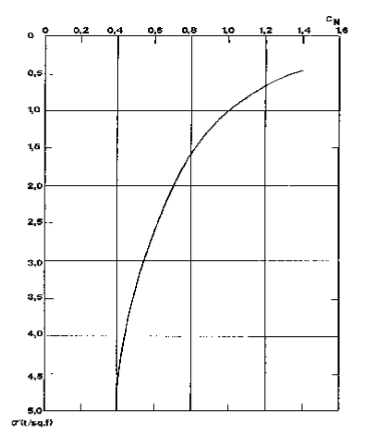
\includegraphics[scale=1]{images/photo2.PNG}
\end{center}

Abaque qui corrige N en fonction de la contrainte verticale au niveau de l'essai et de la densité relative.

\subsection{Corrélations}

\underline{Sables :}

\begin{center}
\begin{tabular}{c|c|c}
    $(N)_{60}$  & $D_r(\%)$     & Compacité \\
    \hline
    0 - 4       & 0-15          & Très lâche \\
    4 - 10      & 15 - 35       & Lâche \\
    10 - 30     & 35 - 65       & Moyennement compact \\
    30 - 50     & 65 - 85       & Compact \\
    > 50        & 85 - 100      & Très compact 
\end{tabular}
\end{center}

\underline{Argiles :}

\begin{center}
\begin{tabular}{c|c|c|c}
    $(N)_{60}$  & $c_u(kPa)$    & Consistance   & Pénétration du pouce \\
    \hline
    0 - 2       & 0 - 12        & Très molle    & > 25 mm \\
    2 - 4       & 12 - 25       & Molle         & \~ 25 mm \\
    4 - 8       & 25 - 50       & Moyenne       & effort modéré \\
    8 - 15      & 50 - 100      & Raide         & \~ 8 mm \\
    15 - 30     & 100 - 200     & Très raide    & ongle \\
    > 30        & > 200         & Dure          & Pas de pénétration
\end{tabular}
\end{center}

Ces méthodes ne sont pas précise mais donne une indication préliminaire de la consistance ou de la densité relative. Beaucoup de géotechniciens la considère comme suffisante. Terzaghi recommande cependant d'autre essai pour des structures "importantes".

\section{Essai de pénétration au cône}

Il en existe deux types : dynamique (DPC) ou statique (CPT).

\subsection{Test de pénétration au cône dynamique (DPC)}

\subsubsection{Description}

Enfoncer une tige munie d'un cône à l'aide d'une masse en chute libre (8kg). Mesurer la profondeur obtenue après chaque coup. On arrête l'enfoncement quand on a un refus, recueillie tous les 10 cm.

Outils adapté aux sols fins contenant peu de gravier et de cailloux (risque d'occasionner un refus). Il a pour avantage d'éviter la réalisation d'excavation ou de trous importants. Utilisé en complémentarité d'un programme de sondage et/ou carottage.

\subsubsection{Déroulement des essais}

On commence parfois l'essai dans un forage pour débuter à une hauteur désirée. On utilise une hauteur de chute et des masses de marteau normalisées (h = 575 mm). 4.6kg en présence de sols mous, 8kg pour les autres. Un cycle à une fréquence de 26 coups à la minute. On peut réaliser de 6 à 10 essais par jour.

Un compteur de coups et un potentiomètre mesurant l'enfoncement permettent d'établir un indice de pénétration [mm/coup]. 

Si le matériaux est lâche, pour éviter l'affaissement et réduire le frottement sur les tiges on utilise un tubage. 

\subsubsection{Analyse des données}

\begin{itemize}
    \item Dresser un profil de pénétration des sols et des matériaux.
    \item Estimer l'épaisseur et la profondeur des couches.
    \item Déduire les propriétés mécaniques des sols (+ variations saisonnières).
    \item Déterminer la profondeur des socles rocheux (proche de la surface).
    \item Détecter des couches de faible consistance (tourbe, argile molle) et des remblais, noyaux,...
    \item Vérifier la profondeur de dégel dans le corps d'une chaussée.
\end{itemize} 

Ils permettent aussi dans le cas de matériaux homogène de connaître l'uniformité de compactage (utilité de contrôle lors de mise en place).

On peut transformer le nombre de coups en terme de résistance unitaire dynamique $q_d$ via une formule de battage.

\subsection{Test de pénétration au cône static (CPT)}

\subsubsection{Introduction}

Il s'agit d'un des outils principal en Belgique et en Hollande. Il fournit la résistance à la pénétration en fonction de la profondeur :

\begin{center}
\begin{tabular}{c|c}
    $q_c = \frac{Q_c}{A_c} $    &   $q_C$ : résistance à la pénétration    \\
                                        &   $Q_c$ : force exercée par le cône   \\ 
                                        &   $A_c$ : section horizontale du cône  
\end{tabular}
\end{center}

\subsubsection{Appareillage}

\begin{itemize}
    \item 25 kN pour les appareils légers portables
    \item 200 kN pour les appareils lourds (ancrage nécessaire et tube évidés (=creux) pour éviter le flambement) (permet de percer certaine couches particulièrement résistante par battage ou vibro-battage).
\end{itemize}

Mesures peuvent être automatique en utilisant une pointe électrique (mesure précise et locale du frottement unitaire ($q_s$) le long du manchon). Les mesure $q_c$ obtenue avec une pointe électrique sont légèrement plus élevée qu'avec une pointe mécanique.

\subsubsection{Déroulement de l'essai et analyse des résultats}

On enfonce la pointe seule sur 4cm à la vitesse de 2 cm/s. On mesure ainsi $Q_c$. En poussant sur le tube, celui-ci vient buter contre la pointe. On peut donc mesurer l'effort total $Q_t$ qui est la somme du frottement latéral cumulé ($Q_s$) et de la réaction à la pointe ($Q_c$). On recommence l'opération tous les 20cm. 

\underline{repère :} $q_{s, argile}$ > $q_{s, sable}$

\begin{center}
    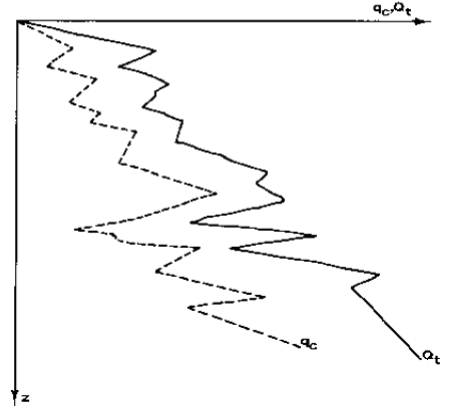
\includegraphics[scale=0.7]{images/photo3.PNG}
\end{center}

On peut finalement définir l'indice de frottement : 

\begin{center}
\begin{tabular}{c|c}
    $ f_r = \frac{q_s}{q_c} 100\% $    &   $f_{r, sable}$ = 0 - 5\%    \\
                                        &   $f_{r, argile}$ = 5 -10\%   
\end{tabular}
\end{center}

\subsubsection{Corrélation à partir du CPT}

\underline{Argiles saturées :}
La vitesse d'enfoncement du cône (2 cm/s) en comparaison à celle de consolidation d'un volume d'argile permet de considérer le sol comme non drainé. On peut donc utiliser les solutions plastiques :

\begin{center}
\begin{tabular}{c|c}
    $ c_u = \frac{q_c - \sigma_{v0}}{N_k} $    &   $N_k$ = 15 - 20 en fonction du type de cône 
\end{tabular}
\end{center}

\underline{Sables :} 
La pénétration est drainée on ne peut donc pas lier les résultats à $c_u$. On s'intéresse à la déformabilité : 

\begin{center}
\begin{tabular}{c|c}
    $E_{50} = 2.5 - 3.5 q_c$    &   $E_{50}$ la déformabilité à 50\% de rupture 
\end{tabular}
\end{center}

\subsection{Piézocone}

Il s'agit d'un essai CPT auquel on a ajouté une mesure de pression interstitielle. La pression est mesurée soit en régime de pénétration, soir à l'arrêt.
Dans le premier cas, la mesure ne correspond pas à la pression d'équilibre dans le sol. En effet, on a une déformation induit par le refoulement et donc une variation de volume (sol contractant ou dilatant).
Dans le second cas, le suivi de la dissipation des surpressions permet d'évaluer le coefficient de consolidation et donc de se faire une idée de perméabilité.

\subsubsection{Surpression interstitielle lors de la pénétration dans un sol sableux :}

La résistance d'un sable dépend de sa compacité. Elle varie fort suivant qu'elle soit supérieur ou inférieur à sa capacité critique.

\underline{Sable dilatant :} Si très compact (dense), le cisaillement induit un déboîtement des grains, on a donc une augmentation de volume. L'augmentation du volume des vides induit une dépression (succion) dans l'eau interstitielle (si non drainé saturé).

\underline{Sable contractant :} Si peu compact (lâche), le cisaillement induit une diminution des vides et le sable se contracte. La diminution du volume des vides induits une surpression dans l'eau interstitielle (non drainé, saturé).

Il existe une compacité intermédiaire qui se fait sans variation de volume (densité critique). Si un sol pulvérulent à une compacité inférieur à la compacité critique, il est potentiellement instable. On risque un phénomène de liquéfaction en cas de cisaillement (séisme, ...).

\subsubsection{Avantage du CPTu par rapport au CPT}

\begin{itemize}
    \item Distinction pénétration drainée, partiellement drainée et non drainée
    \item Correction de la résistance pour tenir compte de la pression interstitielle
    \item Estimation des paramètres d'écoulement et de consolidation
    \item Estimation des conditions hydraulique à l'équilibre
    \item Meilleur caractérisation du type/profil de sol
    \item Meilleur estimation des paramètres géotechniques
\end{itemize}

\subsection{Interprétation des résultats CPT(u)}

\underline{Abaque de Robertson :}

\begin{center}
    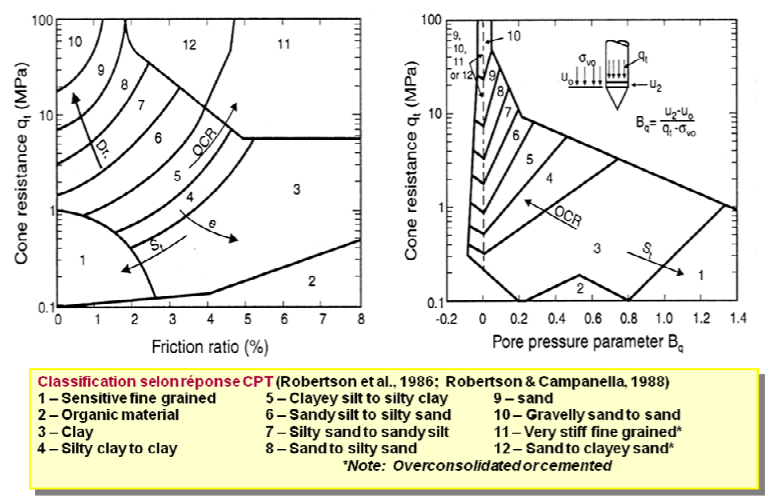
\includegraphics[width=\linewidth]{images/photo4.PNG}
\end{center}

\section{Pénétromètre de poche (PPT)}

Outils rudimentaire pour estimer la résistance à la compression simple ($q_u = 2 c_u$) d'un argile ayant un comportement non drainé. Pratique et utile pour indication rapide mais attention aux matériaux avec $\phi > 0$.

\section{Essai DMT Dilatometrique}

Membrane souple en acier mince ayant un diamètre de 60mm. La membrane est vérinée à une vitesse de 2 cm/s via la technologie CPT. On réalise l'essai tous les 20 à 30 cm. La membrane est gonflée avec de l'azote comprimé. On peu ainsi évaluer : 

\begin{center} $c_u$, $K_0$, OCR, $c_v$, k, raideur du sol \end{center} 

\section{Scissomètre}

Permet de déterminer la résistance au cisaillement non drainé d'une argile saturée. Il s'agit d'une croix soudé à une tige métallique, l'ensemble est enfoncé statiquement dans le sol. On applique un couple pour lui donner une vitesse de rotation w constante. On a un cisaillement du sol de surface cylindrique de hauteur h et de diamètre d (20 - 100mm). On suppose que la contrainte de cisaillement est distribuée uniformément sur le cylindre, on peut donc mesurer le couple nécessaire en fonction de l'angle de rotation. 

\begin{center}
    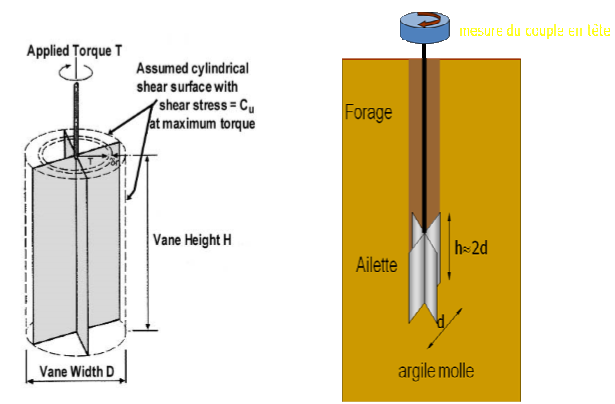
\includegraphics[scale=0.7]{images/photo5.PNG}
\end{center}

\section{Coût-Richesse}

\begin{center}
    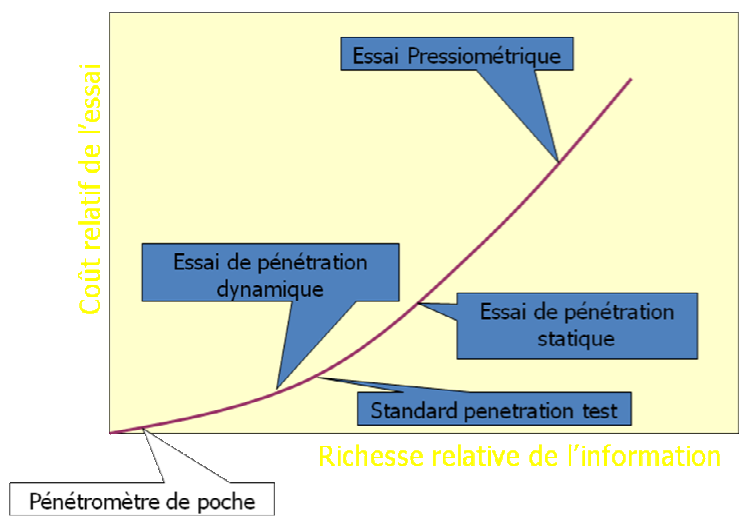
\includegraphics[scale=0.7]{images/photo6.PNG}
\end{center}

\newpage

\part{Le pressiomètre}

\section{Essai pressiométrique}

Essai de chargement du sol, consiste à dilater radialement au sein du sol une sonde cylindrique et ainsi déterminer la relation entre la pression appliquée et le déplacement de la paroi de la sonde.

\begin{center}
    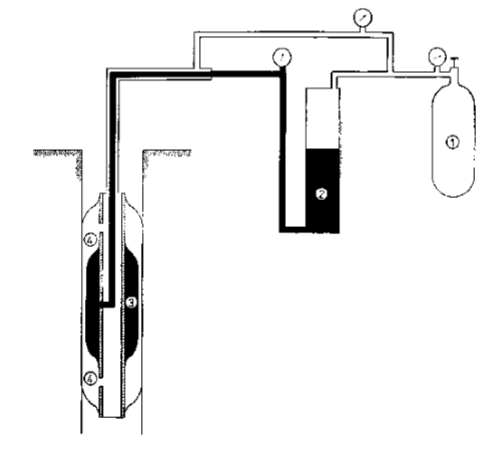
\includegraphics[scale=0.7]{images/photo7.PNG}
\end{center}

\subsection{La sonde pressiométrique et son contrôle}

Il en existe deux type : 

\subsubsection{La sonde à gaine souple}

Trois cellules cylindriques à section circulaire et de même axe, agissant simultanément sur la paroi du forage pendant l'essai :
\begin{itemize}
    \item Une cellule centrale de mesure (diamètre d, longueur $l_s$) capable de se déformer dans un forage (diamètre $d_t$) et d'appliquer une pression uniforme au sol (injection de liquide incompressible).
    \item deux cellules de garde (diamètre d, longueur $l_g$) situées de part et d'autre de la cellule centrale et destinées à transmettre au sol la même pression que la cellule centrale. Elles sont gonflées à l'aide d'un gaz. 
\end{itemize}

La pression dans les cellules de garde doit être légèrement inférieur à celle de la cellule centrale de manière a éviter un décollement de la gaine qui recouvre la membrane.

\begin{center}
    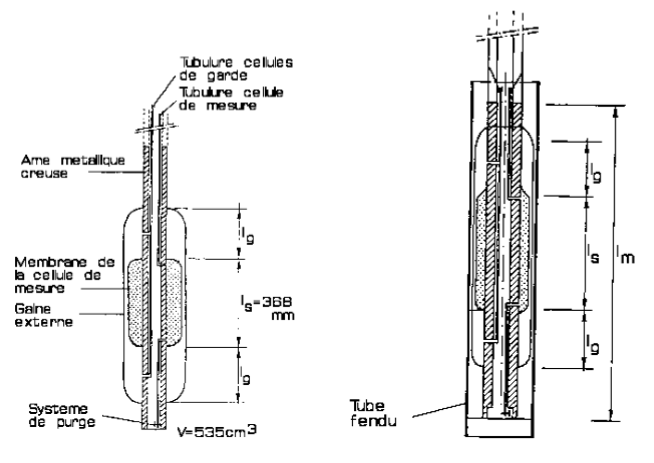
\includegraphics[scale=0.7]{images/photo8.PNG}
\end{center}

\subsubsection{La sonde avec tube lanterné}

C'est une sonde du même type que la sonde à gaine souple, mais de diamètre 44mm. Elle est placée à l'abri d'un tube de diamètre extérieur d=63mm, fendu longitudinalement selon 6 génératrices équidistantes et sur une longueur $l_m$ telle que :

$$ l_m > 1.4 (l_s + 2l_g) $$

Elle peut être insérée par battage dans des sols résistants (sablo-graveleux - sableux immergés). On arrête le battage pour une résistance de 100 coups pour 10 cm d'enfoncement (1 kN de 40cm). Il faut faire attention au type de sol (possible refoulement si le sol est trop mou). Elle est tolérée dans des limons ou des sables immergé mais déconseillée pour des argiles et limon au dessus de la nappe.

Si on opte pour une solution "forage", on doit obligatoirement effectuer une injection de bentonite, utiliser un train de tige rigide (fouettement latéral). La paroi du forage doit être intacte et son diamètre de 3 à 6 mm supérieur à celui de la sonde (maximum).

Le contrôleur pression-volume est composé d'un système de mise en pression/dilatation de la sonde et d'un conditionneur-indicateur (et éventuellement d'un dispositif de stockage des données pour faire des analyse dans le temps).

\subsection{Sondage pressiométrique}

Il s'agit d'un forage pressiométrique suivit d'un ou plusieurs essais pressiométrique. L'expression "sondage" exprime à la fois la technique et la représentation de l'ensemble des paramètres pressiométriques réalisé au cours d'un même forage. Cela permet :
\begin{itemize}
    \item Apprécier la stratigraphie
    \item Orienter le choix des fondations
    \item Dimensionner les fondations
    \item Évaluer les tassements et autres déformations
\end{itemize} 

\subsubsection{Profil et nature du sol}

Il existe des catégories significatives de sols ou de roches. Dans le calcul de la capacité portante des fondations superficielles on n'en considère que trois : Les sols fins cohérents, les sols granuleux et les roches tendres ou fissurées. Par contre, pour des fondations profondes, on divise les roches tendres ou fissurées en craie (et marnes) ou en roches altérées (ou fragmentées).

\subsubsection{Forage pressiométrique}

Il s'agit du procédé qui permet d'introduire la sonde dans le sol. Il existe deux techniques : le forage préalable et l'introduction directe de la sonde.

Choix dépend de la nature et de l'état des terrains rencontrés afin de remanier le moins possible. L'attention se porte ici sur le sol à l'extérieur du forage (à l'inverse d'un prélèvement). Les longueur maximales de forage destructif à réaliser avant l'introduction de la sonde sont fonction de la nature des sols, de leur état et de l'existence ou non d'une nappe.

\subsubsection{Influence du mode de forage}

Il y a différents problèmes sur les valeurs pressiométriques du à la mise en oeuvre : 

La qualité des parois du forage a une influence sur la valeur du module pressiométrique. il faut que les parois soient intactes, que le forage soit bien calibré et que les fluides d'injections ne polluent pas le sol.

Dans un sol mou, seul la tarière manuelle permet de remplir ces conditions. Dans les sols meubles (plus compact) les forages par rotation mécanique sont acceptables (les battages sont défectueux). Valide si le rapport $\frac{P_l}{P_f}$ se limite à 1,7.

De nouveaux tests on été effectué sur des marnes et argiles raides. Les auteurs concluent que pour ces type de sols, quel que soit l'outil de forage utilisé, les caractérisation pressiométrique sont les même à : 
\begin{itemize}
    \item 20\% près pour les modules pressiométriques,
    \item 10\% près pour les pressions limites,
    \item 10\% près pour les pressions de fluage,
    \item 15\% près pour les rapports $E_M/P_l$
\end{itemize} 

\subsection{Essai pressiométrique Ménard}

La réalisation de l'essai doit suivre immédiatement l'opération de forage. Un délai de repos est accetable si on maintient l'interface sol-onde intact.

Cet essai nous fourni :
\begin{itemize}
    \item $p_l$ : pression limite
    \item $E_M$ : module pressiométrique
\end{itemize} 

\subsubsection{Programme de chargement de l'essai pressiométrique}

\begin{center}
    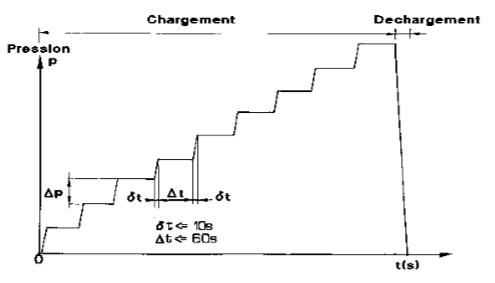
\includegraphics[scale=1]{images/photo9.PNG}
\end{center}

On augmente progressivement la pression par palier identique que l'on garde constant pendant une durée $\Delta t$ fixée ($\Delta t < \delta t$). Le déchrgement se fait sans palier.

\subsubsection{Volume de la cellule centrale de mesure de la sonde pressiométrique}

Il s'agit théoriquement d'un cylindre de volume $v_s$. On peu déterminer ce volume expérimentalement pour une sonde particulière. On l'introduit dans un tube de calibrage en acier et on fait une mise en pression par palier. Chaque pression est maintenue pendant une durée de 60s. On mesure le volume injecté en fin de palier afin de tracer la courbe $V=f(p)$:

\begin{center}
    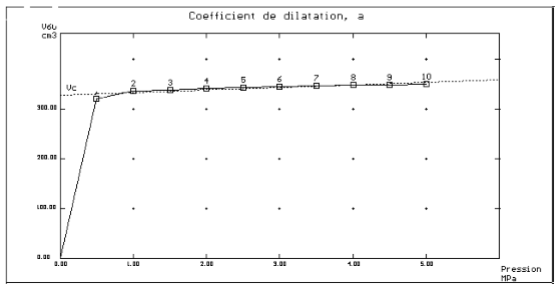
\includegraphics[scale=1]{images/photo10.PNG}
\end{center}

Il faut entre 6 et 14 paliers pour que l'essai soit normalisé. On considère pour chaque pression la plus grande pression exercée et on la divise par 10 ($p_l/10$).

Par convention, le volume de la cellule centrale de mesure a pour valeur :

\begin{center}
\begin{tabular}{c|c}
    $V_s = \frac{\pi l_s d_i^2}{4} - V_c$ 
        &   $d_i$ : diamètre intérieur du tube de calibrage  \\
        &   $l_s$ : longueur du tube de calibrage (à vérifier) \\
        &   $V_c$ : volume de liquide injecté dans la sonde pour qu'il y ait un contact entre le tube et la sonde  
\end{tabular}
\end{center}

On calcul un coefficient de dilatation ou gonflement ($\alpha$) :

\begin{center}
\begin{tabular}{c|c}
    $\alpha = \frac{\Delta V}{\Delta p}$ 
        &   $\Delta V$ : différence de volume  \\
        &   $\Delta p$ : différence de pression 
\end{tabular}
\end{center}

Il permettra de déterminer le volume effectivement introduit dans la sonde : 

\begin{center}
\begin{tabular}{c|c}
    $V = V_r - \alpha p_r$ 
        &   $alpha$ : coefficient de dilatation  \\
        &   $V_r$ : volume lu 
\end{tabular}
\end{center}

\subsection{Mesure a effectuer pour l'établissement de la courbe pressiométrique}

A chaque profondeur, on mesure l'évolution de la déformation de la cavité pressiométrique en fonction de la pression appliquée sur le sol. On le fait environ tous les mètres. On obtient un volume V et une pression p qui nous donneront les paramètres pressiométriques. Il faut les corriger avec :
\begin{itemize}
    \item $p_h$ : la charge hydraulique
    \item $p_e$ : la résistance propre à la sonde
    \item les dilatations parasites
\end{itemize} 
On obtient la courbe pressiométrique corrigée.

\subsubsection{Correction de charge hydraulique}

Il y a une pression hydrostatique existante entre la prise de pression et le milieu de la sonde :
\begin{center}
\begin{tabular}{c|c}
    $p_h = \gamma_i (z_c - z_s)$ 
        &   $\gamma_i$ : poids volumique du fluide injecté  \\
        &   $z_s$ : cote pressiométrique du milieu de la cellule  \\
        &  $z_c$ : cote pressiométrique du conditionneur de pression 
\end{tabular}
\end{center}

 \subsubsection{Correction de résistance propre de la sonde}
 
 Il faut tenir compte de la résistance propre ($p_{er}$) de l'ensemble membrane-gaine et éventuellement du tube lanterné. 
 Pour déterminer la résistance propre de la sonde, On la place hors sol, à l'air libre et on effectue un essai d'expansion dans les même condition qu'un essai, par palier (60sec, ...). L'essai se déroule par pas de pression d'environ le dixième de la pression maximale ($p_{el}$) pour pouvoir faire 10 paliers, jusqu'à ce qu'on ait injecté un volume V = 1.2 $V_s$. on obtient ainsi une courbe pression-volume d'étalonnage. Par convention, $p_e$ est la pression liquide injecté à la fin du test.
 
 \subsubsection{Courbe pressiométrique corrigée}
 
 Une courbe pressiométrique est une représentation graphique d'un volume de liquide injecté dans la sonde en fonction de la pression V = f(p). ou V est le volume injecté à la fin de chaque palier de pression p.
 
 La courbe corrigée V = f(p) est tracé pour chaque essai en fin de palier avec : 
 
\begin{center}
    $ p = p_r + p_h - p_{er} $ [kPa] ou [MPa]
    $V = V_r - \alpha p_r$  [$cm^3$] 
\end{center}

\begin{center}
    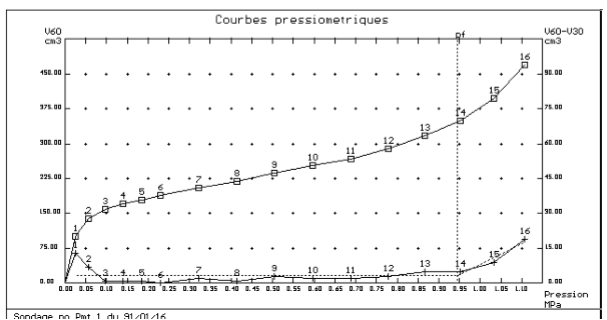
\includegraphics[scale=1]{images/photo11.PNG}
\end{center}

On observe ci-dessus, la courbe pressiométrique et la courbe de fluage (incrément de volume gagné par la cellule entre 30 et 60 sec en fonction de la pression de chaque palier).

On divise une courbe pressiométrique en trois parties :
\begin{itemize}
    \item I  : mise en contact paroi sonde
    \item II : comportement pseudo élastique du sol (permet de définir le module pressiométrique), approximation linéaire
    \item III: phase de grand déplacement de la paroi du forage
\end{itemize}

\section{Paramètres pressiométriques}

\subsection{Pression de fluage}

On obtient la pression de fluage ($p_f$) en exploitant le diagramme du fluage (présenté ci-dessus). Lorsque la pression est maintenue constante, on détermine une variation de volume correspondant à un phénomène de fluage. On distingue ainsi deux gammes de pressions correspondant à une pshase pseudo élastique et à une phase plastique.

\begin{center}
\begin{tabular}{c|c}
    $\Delta V^{60}_{30} = V_{60} - V_{30}$ 
        &  $\Delta V^{60}_{30}$ : variation de volume injecté dans la cellule centrale  \\
        &  $V_{60}$ : volume en t = 60  \\
        &  $V_{30}$ : volume en t = 30 
\end{tabular}
\end{center}

\subsection{Pression limite pressiométrique}

C'est la pression qui entraîne le doublement du volume de la cellule centrale lorsque celle-ci entre dans la phase pseudo-élastique. Elle correspond à un volume : $V = V_s + 2V_1$ et s'exprime en kPa ou MPa.

Lors d'un essai d'expansion, si le volume injecté est inférieur à ce volume alors on applique la méthode suivante pour calculer la pression limite : 

\begin{itemize}
    \item si le nombre de palier de pression au dela de la pression $p_2$ est inférieur ou égal à 2 alors :
\begin{center}
\begin{tabular}{c|c}
   $ p_l = 1.7p_f - 0.7 \sigma_{HS} $
        &  $\sigma_{HS}$ : contrainte horizontale initiale 
\end{tabular}
\end{center}

    \item si le nombre de palier de pression au delà de la pression $p_2$ est supérieur à 2 alors : 
    
\begin{center}
\begin{tabular}{c|c}
   $Y = (V)-1 = A p + B$
        &  A et B sont des coefficients
\end{tabular}
\end{center}

\begin{center}
$p_l = \frac{B}{A}+\frac{1}{A(V_s + 2V_1)}$

$p_l = 1.7 p_f - 0.7 \sigma_{HS}$
\end{center}
En absence de donnée, on utilise $\gamma = 15 kN/m^3$ et $K_0 = 0.5$.

\end{itemize} 

\subsection{Pression limite nette}

C'est la pression limite comptée par rapport à la contrainte totale horizontale régnant dans le sol avant introduction de la sonde au même niveau: 

\begin{center}
$ p_l* = p_l - \sigma_{HS}$ \\
$\sigma_{HS} = k_0(\sigma_{VS}-u_s)+u_s$
\end{center}

En supposant un nappe phréatique au niveau du sol on obtient :

\begin{center}
\begin{tabular}{c|c}
   $p_l* = p_l - (\gamma_w + K_0\gamma')h$
        &  h: profondeur de la sonde \\
        &  $\gamma'$: poids volumique déjaugé du sol \\
        &  $K_0$: coefficient des terres au repos 
\end{tabular}
\end{center}

Généralement :
$\gamma'$ = 5.5 $kN/m^3$, $K_0$ = 1 pour un sol très lâche.

$\gamma'$ = 11 $kN/m^3$, $K_0$ = 0.5 pour un sol compact.

\subsection{Pression de fluage nette}

C'est la pression de fluage comptée par rapport à la contrainte totale horizontale régnant dans le sol avant introduction de la sonde au même niveau :

$$ p_f*=p_f - \sigma_{HS}$$

\subsection{Plage pseudo élastique}

La courbe pressiométrique corrigée est constituée d'une succession de couples de mesures $(p_i, v_i)$ entre lesquels on a une pente $m_i$. On cherche la valeur m la plus faible. Par définition, la plage pseudo élastique d'un essai pressiométrique est constitué de l'ensemble des segments qui ont une pente m inférieru à $\beta$ fois la pente $m_E$ la plus faible : 

$$ m \leqslant \beta m_E $$

$\beta$ permet de tenir compte des incertitude de mesures :

\begin{center}
\begin{tabular}{c|c}
   $\beta = 1 + \delta p \frac{p_{E'}+p_E}{p_{E'}-p_E}+\frac{2\sigma_v}{v_{E'} - v_E}$
        &  $\delta_p$ : erreur relative sur la mesure en pression 1/100 \\
   $\approx 1.5$    
        &  $\delta_v$ erreur absolue sur la mesure du volume injecté 
\end{tabular}
\end{center}

\subsection{Module pressiométrique Ménard}

Ménard a repris le développement de lamé qui résout le problème du cylindre élastique soumis à des pressions interne et externe différentes (démo p15 - 16 syllabus sur le pressiomètre). 

Par application de la solution de Lamé à un cylindre à paroi infiniment épaisse de rayon intérieur r, Ménard a donc proposé de définir le module pressiométrique par référence au module de Young, ce qui exige de connaître ou de postuler une valeur du coefficient de Poisson : 

$$ \frac{\delta r}{r} = \frac{1 + \nu}{E_M} \delta p $$

Par conséquence, Ménard propose de déduire expérimentalement le module pressiométrique sur base des points de mesure définissant l’extension de la phase pseudo-élatique, par la formule : 

\begin{center}
\begin{tabular}{c|c}
   $E_M = 2(1+\nu)(v_s+\frac{v_1 + v2}{2})\frac{p_2-p_1}{v_2-v_1}$
        &  $\nu$: coefficient de poisson (0.33) \\
        &  $v_s$: volume de la cellule centrale \\
        &  $p_2,v_2$: pression et volume à l'extrémité de la plage pseudo élastique \\
        &  $p_1,v_1$: pression et volume à l'origine de la plage pseudo élastique \\
        &  $p_2$: doit être inférieur ou égal à $p_f$ [MPa] 
\end{tabular}
\end{center}

\subsection{Pression limite théorique}

Le résultat de lamé ne peu être considéré que dans la phase pseudo élastique car le sol n'est pas élastique isotrope. On peu toutefois complétée le modèle par une étude théorique des contraintes de déformations au delà de la théorie de l'élasticité. Il faut introduire des relations constitutives caractérisant le comportement du matériau sous grandes déformations :

\begin{itemize}
    \item Argiles non drainée : tresca : $\sigma_p - \sigma_{\theta} = DEV = 2S_u(ND)$
    \item Sables drainé : Mohr-Coulomb : 
    $\sigma_p - \sigma_{\theta} = 2\frac{sin\phi'}{1+\sin\phi'}\sigma_p + 2c'\frac{cos\phi'}{1+sin\phi'}(D)$
\end{itemize} 

Dans le cas de la plasticité parfaite, le déviateur des contraintes reste constant alors que le volume ne varie plus : 

$$ DEV = V(1 +\frac{V}{V_0}) \frac{dp}{dV} $$

Dans le cas d’une argile parfaitement élasto-plastique caractérisée par une résistance au cisaillement non drainé ($S_u$) la pression croît indéfiniment lorsque la cavité se dilate indéfiniment : 

$$ P = \sigma_{h0} + S_u(1+ln\frac{G}{S_u})+S_u ln\frac{\Delta V}{V}$$

Il est en outre intéressant de noter que, dans un matériau élasto-plastique avec critère de rupture de Tresca, la pression limite dépend de G/Su. Ce rapport adimensionnel, parfois dénommé indice de rigidité (Ir) en cisaillement est alternativement exprimé sous la forme de son inverse : $\gamma_r$, qui exprime la déformation angulaire délimitant le domaine élastique du domaine plastique dans la loi elasto-plastique. Cette formule permet de comprendre que la pression limite dans ce cas dépend au premier chef de la résistance au cisaillement Su de l’argile, mais aussi au second degré de sa raideur relative.  Pour une valeur moyenne de 250 de l’indice de rigidité, l’équation de Vesic conduit à une valeur théorique de p*l/Su de l’ordre de 5.5.

\section{Relation impliquant les paramètres pressiométriques}

\subsection{Relations entre pression limite et paramètre intrinsèques des sols}

Nous avons vu qu’il est possible, sur base des théories fondamentales de la mécanique des sols et au prix d'un certain nombre d'hypothèses simplificatrices, d'établir des relations théoriques entre les paramètres classiques de l'élasticité et EM, d'une part, et entre les paramètres classiques de la plasticité (p.ex. critère de Coulomb) et pl d'autre part.

Lorsqu'il s'agit des sols à caractère granuleux, ces relations sont assez mal vérifiées expérimentalement. Pour les sols cohérents ($c_u=S_u$), par contre la vérification expérimentale est meilleure et les relations approximatives obtenues sont: 

\begin{center}
$c_u \le 0.5 bar \to c_u = \frac{p_l*}{5.5}$ et $p_f = 3.2 c_u$\\
$\frac{p_l}{p_f} = 1.72$\\
$c_u > 0.5 bar \to c_u = \frac{p_l*}{10}+0.25$
\end{center} 

Pour des sols pulvérulents, on a l'expression approchée :

$$ p_l* 2.5 * 2^{\frac{\phi'-24}{4}}$$

\subsection{Ratio entre module pressiométrique et pression limite}

Selon Ménard : 
\begin{itemize}
    \item $E_M/p_l < 5$ : argiles remaniées ou triturées 
    \item $5<E_M/p_l < 8$ : argiles sous-consolidées 
    \item $8<E_M/p_l < 12$ : argiles normalement consolidées 
    \item $12 < E_M/p_l < 15 $ : argiles légèrement surconsolidée
    \item $E_M/p_l > 15 $ : argiles fortement surconsolidées
\end{itemize}

On peu observer que si $E_M/p_l$ vaut environ 10, le sol est normalement consolidé. Une valeur plus élevée, le sol est surconsolidé. C’est pourquoi on représente parfois le module pressiométrique et la pression limite sur le même profil avec un facteur d’échelle relatif de 10.

\subsection{Relation entre le module oedométrique et le module pressiométrique}
 
\begin{center}
\begin{tabular}{c|c}
   $E_{oed} = \frac{E_M}{\alpha}$
        &  $\alpha$: coefficient de structure 
\end{tabular}
\end{center}

\begin{center}
    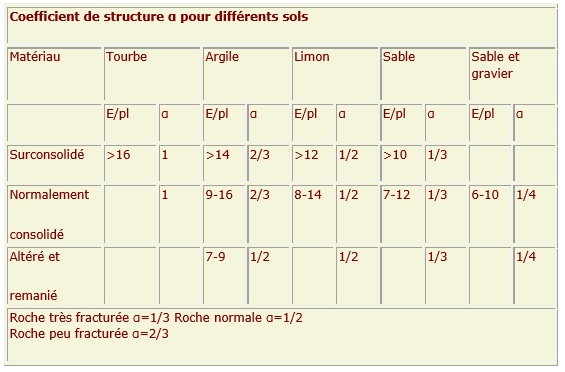
\includegraphics[scale=1]{images/photo13.PNG}
\end{center}

\subsection{Relation entre $p_l$ et $q_c$}

 Le rapport qc/pl vaut 3 pour les argiles, 6 pour les limons, 9 pour les sables et graviers et 12 pour les sables et graviers denses. - Van Wambeke \& al. (1982)
 
 \subsection{Valeurs pressiométriques caractéristiques}
 
 \begin{center}
    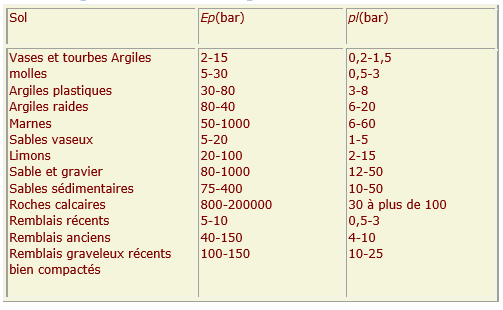
\includegraphics[scale=1]{images/photo14.PNG}
\end{center}

On constate que l'établissement de formules d'interprétation et de corrélation avec d'autres paramètres est surtout satisfaisant dans les sols cohérents. Cependant, on constate que les calculs de capacités portantes et de tassements de fondations sur sols pulvérulents, basés sur les essais pressiométriques, sont également très satisfaisants. 

\section{Pressiomètre AutoForeur (PAF)}

\begin{itemize}
    \item L'appareil consiste essentiellement en un dilatomètre à une seule chambre précédé d'un carottier à paroi mince portant la cellule de mesure. La carotte est détruite au fur et à mesure de la pénétration dans le terrain par une tarière à ailette mue par un arbre de rotation et par une injection de fluide qui remonte par l'intérieur et non entre la membrane et le terrain. La trousse coupante du carottier est biseautée vers l'intérieur. 
    \item la mise en place de la sonde dans le terrain se fait par autoforage, c'est-à-dire que la sonde fait elle-même son trou.  Le carottier à paroi mince portant sur les flancs des appareils d'essais ou de mesure est mis en place dans le terrain par vérinage, par battage ou par vibro-battage. Au fur et à mesure de l'enfoncement dans le terrain, le sol qui pénètre à l'intérieur du carottier est désagrégé par un outil rotatif  
    \item Les sédiments sont remontés jusqu'à la surface grâce à l'injection d'un fluide sous pression à l'intérieur du carottier. Cette mise en place perturbe très peu le sol. Cependant, la pression du fluide de forage doit être suffisamment faible pour éviter le claquage du sol, mais suffisamment élevée pour permettre l'évacuation des déblais.  Le PAF peut être utilisé pour des granulométries inférieures à la dimension d'une grave. L'opérateur doit être particulièrement attentif au risque d'éboulement des sols pulvérulents, conduisant à la perte de la sonde.
    \item le système de mise en charge pour l'essai d'expansion peut, suivant les propriétés du sol à étudier être à déformation ou à pression contrôlée.  Le module de mesure est constitué par une sonde cylindrique dilatable monocellulaire. La membrane constituant la cellule de mesure est située dans le prolongement de la trousse coupante du carottier. 
    \item La sonde est descendue dans le sol à volume constant. Pendant cette phase, on note les variations de pression dans la sonde qui agit alors comme un capteur, et on contrôle ainsi la qualité de la mise en place. Une fois arrivée au niveau à tester, la sonde est immobilisée et on effectue les opérations suivantes: 
    \begin{itemize}
        \item mesure de la pression horizontale totale $p_{0h}$; 
        \item essai d'expansion proprement dit, qui permet la détermination in situ de propriétés élémentaires fondamentales telles que la résistance non drainée. 
    \end{itemize}
\end{itemize}

\newpage

\part{Méthode observationnelle et mécanique des ondes dans les pieux}

\section{Démarche observationnelle}

\subsection{Introduction}

Un modèle mathématique n'est jamais complètement fiable, il n'est qu'une représentation partielle, idéalisée et incomplète. Un chantier se déroule in situ, en domaine réel. Il faut donc prévoir, dans la conception même du projet, un programme d'observation in situ pour vérifier dans quelle mesure la théorie correspond à la pratique. Le modèle se place toujours du côté de la sécurité : coefficient de sécurité, choix des caractéristiques hydro-mécaniques, ...

On présente le problème sous trois aspects :

\begin{itemize}
    \item Main concerns
    \item Expectations
    \item Time (money)
\end{itemize}

Il faut s'attendre à ce que le modèle change (nouveau paramètres). En effet, la perception de l'ingénieur gagne en maturité et s'affine durant le chantier. Il faut donc constamment imaginer des modifications et en évaluer l'intérêt dans le but de réduire l'impact des aléas géotechniques. 

\subsection{Mise en oeuvre}

Introduite par Terzaghi et Peck en 1960, elle consiste à intégrer au processus de conception de l'ouvrage, les observations effectuées dès le début des travaux. Cette méthode est applicable à condition d'avoir des données observées fiables et pertinentes.

\subsubsection{Étapes de mise en oeuvre de la méthode observationnelle}

\begin{itemize}
    \item On commence par définir le milieu (une caractérisation de l'expérience): Milieu, géométrie, conditions limites,...
    \item Imagine les résultats à venir pour pouvoir les comparer au modèle et se donner une marge d'erreur.
    \item Établir un design type basé sur des hypothèses, c'est à dire sur les anticipations faites et sur les déviations acceptées.
    \item Sélectionner les quantités qui doivent être observées pendant l'expérience et calculer la distribution des résultats (anticiper $\to$ comparer).
    \item On travail en temps réel donc il est important de prévoir à l'avance les conséquences provoquées par le changement de certains paramètres.
    \item Rédéfinir les conditions expérimentales et redessiner les expériences en cas de besoin.
\end{itemize}

\section{Essais statiques sur pieux}

\subsection{Essai de mise en charge statique}

Permet de récolter des mesures caractérisant le comportement réel d'un pieu tel que réalisé, généralement sous charge axiale.

 \begin{center}
    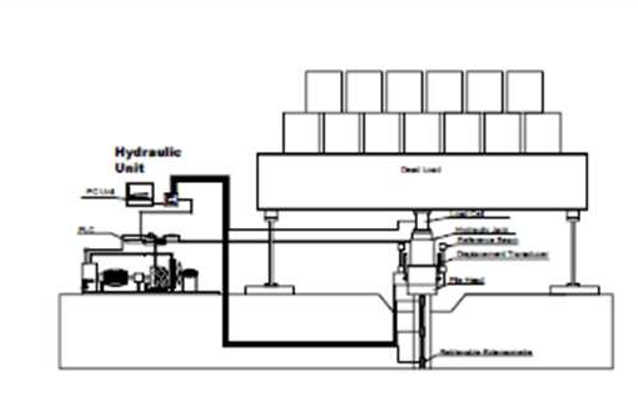
\includegraphics[scale=1]{images/photo15.PNG}
\end{center}

Le pieu est surmonté d'un dé en béton armé dans lequel sont encastrées trois poutrelles de section égale ou supérieur à UPN 120 d'une longueur utile d'au moins 5m, disposées à 120\degree l'une de l'autre. La charge est appliquée sur le pieu de façon statique au moyen d'un vérin hydraulique (par un lest, tirants d'ancrage précontraints, pieux de traction soit par combinaison des moyens précédents). 
\begin{itemize}
    \item Dans le cas du lest, il faut éviter tout risque de déversement à la mise en place du poids mort (surcharge = 1.2x la charge maximale à appliquer).
    \item Dans le cas des ancrages et pieux de traction, la sollicitation exercée sur ceux-ci doit rester sous leur charge de rupture (ancrage et pieux implantés à un distance d'au moins 4m).
\end{itemize}

La charge est transmise au pieu par un vérin indépendant du système de chargement par l'intermédiaire d'une plaque en acier. L'entrepreneur veille à assurer une co-axialité du piston du vérin et du pieu. L'effort appliqué peut être obtenu en multipliant la pression lue au manomètre par la section nominale du vérin (on peu aussi utiliser un dynamomètre calibré). 

Les déformations en tête du pieu sont enregistré au moyen de trois comparateurs fixés aux extrémités des poutrelles. On les places a égale distance de l'axe du pieu. Les poutrelles sont totalement indépendantes du système de chargement et leur niveaux topographiques sont régulièrement relevé durant la mise en charge du pieu. Elles sont protégés contre l'action du vent, du soleil et des variations de température.

\subsection{Extensomètre ou jauge de déformation}

Permet de traduire la déformation d'une pièce à laquelle l'extensomètre est solidarisé. une jauge consiste en des spires rapprochées, fabriqué à partir d'une feuille métallique et d'un isolant.

 \begin{center}
    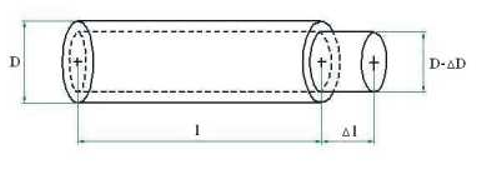
\includegraphics[scale=1]{images/photo16.PNG}
\end{center}

\begin{center}
\begin{tabular}{c|c}
   $R = \rho \frac{l}{A} = \rho \frac{4 l}{D^2 \pi}$
        &  $\rho$: résistivité du conducteur \\
        &  $l$: longueur \\
        &  $A$: aire de sa section \\
        &  $D$: diamètre de la section 
\end{tabular}
\end{center}

Après une déformation axiale $\Delta l$ on peut exprimer la variation relative de la résistance par :

\begin{center}
\begin{tabular}{c|c}
$ \frac{\Delta R}{R_0} = k \frac{\Delta l}{l_0} = k \epsilon_l $
        &  $k$: sensibilité du capteur \\
        &  $\epsilon_l$: variation relative de longueur \\
        &  $R$: résistance 
\end{tabular}
\end{center}

On peut également déterminer une déformation unitaire $\epsilon$ avec un comparateur de précision qui mesure le déplacement relatif $\Delta l$ entre deux points, qui constitue alors la base $L_0$ de mesure.

\underline{Théorie de l'élasticité :}
\begin{center}
\begin{tabular}{c|c}
$ F = E A \epsilon $
        &  $E$: module \\
        &  $A$: section \\
        &  $F$: force 
\end{tabular}
\end{center}

En équipant le fût du pieu d'extensomètres, il devient possible de suivre l'évolution de son effort interne de compression axiale. On observe sur le diagramme que l'effort est maximal en tête de pieux et qu'elle s'amenuise avec la profondeur. Ceci est normal étant donné que la force est reprise par le frottement latéral s'accumulant le long du fût. 

 \begin{center}
    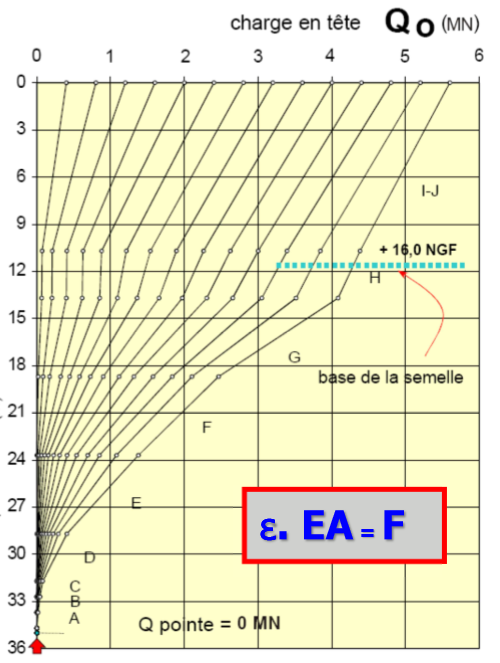
\includegraphics[scale=0.5]{images/photo17.PNG}
\end{center}

Il est difficile de déterminer un E exact pour le béton. Sa relation contrainte déformation n'est pas linéaire et on a observé que la densité augmentait avec la profondeur du fût grâce au poids de la colonne au-dessus. Il est donc normal que la résistance et donc le module du béton croisse de la tête à la base du pieu. Il est également difficile de déterminer A pour un pieu moulé dans le sol, la surface n'est pas régulière.

\subsection{Cellule d'Osterberg}

Il s'agit d'un système d'exploitation de cellules intégrées dans un pieu préfabriqué ou foré. Si la cellule occupe la base (utile pour un pieu portant à la base), elle provoque (en gonflant) un frottement négatif, ce qui fait remonter le fût. Si elle est situé dans une position intermédiaire (utile pour un pieu flottant), elle induit l'équivalent d'un effort de compression interne au pieu ("O-cell"). On poursuit le test jusqu'à l'apparition d'un des phénomènes suivants :
\begin{itemize}
    \item la résistance ultime au frottement latéral est atteinte,
    \item résistance ultime de la base est atteinte,
    \item la capacité de l'O-cell est atteinte.
\end{itemize}

On mesure le déplacement via deux tiges accessible depuis la surface. Une en dessous de la cellule, l'autre au dessus. En mesurant le mouvement et la compression du segment supérieur du fût on détermine le mouvement vers le bas du segment inférieur.

 \begin{center}
    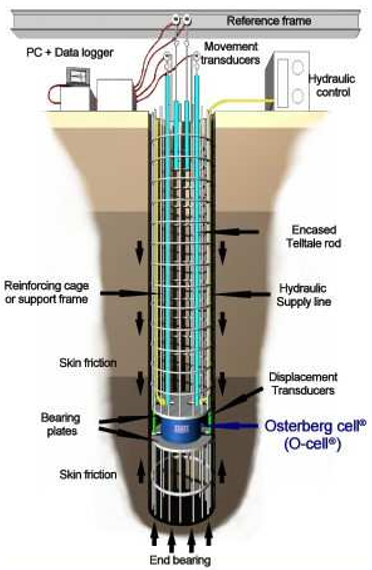
\includegraphics[scale=1]{images/photo18.PNG}
\end{center}

On peu le combiner avec une charge en tête pour augmenter la capacité de l'essai ou en ajoutant une jauge pour mesurer la distribution des charges. On peu obtenir des informations sur les charges limites de fluage, du frottement latéral et sur la résistance de pointe. 

Lors de l'exploitation des résultats, il ne faut pas perdre de vue le sens de mobilisation de la résistance au frottement latéral : 

 \begin{center}
    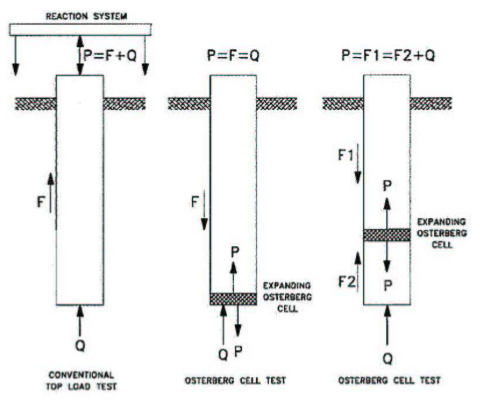
\includegraphics[scale=1]{images/photo19.PNG}
\end{center}

\section{Essais dynamique et cinétique sur pieux}

\subsection{Essai dynamique}

La méthode de mise en charge dynamique des pieux se base sur l'analyse de la réponse impulsionnelle d'un pieu sous l'impact d'une masse en chute libre (limite : 4 tonnes jusqu'à 2m). On obtient ainsi une courbe de mise en charge telle qu'avec un moyen de mise en charge statique plus lourd, long et coûteux. 

\begin{itemize}
    \item La force est mesurée par la technique des jauges amovibles de déformation,
    \item Le mouvement est mesuré à l'aide d'un accéléromètre.
\end{itemize}

L'essai dynamique induit des ondes mécaniques. Il y a deux familles d'essais :

\begin{itemize}
    \item haute énergie (high-strain): déformation et donc contraintes proche de celle amenant à la rupture du béton.
    \item faible énergie (low-strain): non destructif et donc contraintes faibles.
\end{itemize}

\subsection{Essai statnamic}

On place une masse sur le pieu, entre le pieu et la masse est interposé un explosif. La détonation propulse la masse en hauteur en trouvant réaction sur la tête du pieu. La détonation génère un effort interne au système masse-pieu pendant une durée de l'ordre de 100 ms. On mesure à nouveau la force et l'accélération au moyen d'un dynamomètre et d'un accéléromètre. 

On observe également le déplacement vertical du pieu (avec un théodolithe). On intègre l'accélération pour avoir la vitesse et ensuite le déplacement. On a donc deux mesure du déplacement (très utile pour vérifier les infos).

La distinction entre statique, statnatic ou dynamique est la durée de l'impact.
\begin{itemize}
    \item statique : palier de charge d'ordrde heure/jour,
    \item statnatic : durée de chargement 50-100 ms,
    \item dynamique : environ 10 ms
\end{itemize} 

Le comportement du sol dépend de la vitesse de chargement ou de déformation, on obtient donc des résultats différents qu'il faut pouvoir convertir. Le plus représentatif est l'essai statique qui implique le long terme.

\subsection{Instruments mesurant un mouvement transitoire}

\subsubsection{Accéléromètre}

Basé sur la loi fondamentale de la dynamique : $F = ma$. Ces capteurs exploitent l'égalité entre la force d'inertie de la masse sismique du capteur et une force de rappel appliquée à cette masse.

\begin{itemize}
    \item Accéléromètre non asservi (faibles accélération et les basses fréquences) est un système masse-ressort dans laquelle la masse introduit une composante inertielle dont l'effet est mesuré par compression du ressort.
    
    \begin{center}
        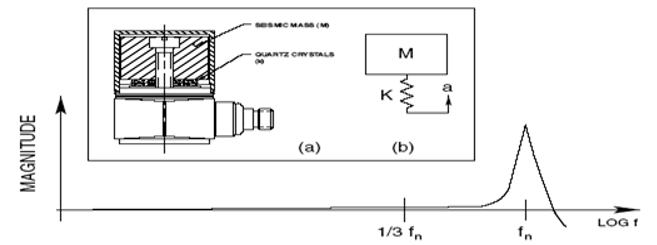
\includegraphics[scale=1]{images/photo20.PNG}
    \end{center}
    
    Lorsque le support subit une accélération, le support va se déplacer tandis que la masse va avoir tendance à rester à sa position de départ. Cette différence de déplacement va forcer le ressort à se comprimer, cela induira un effort sur la masse qui va alors suivre le mouvement du support. En mesurant simplement le déplacement de la masse m par rapport à son support, c'est à dire la compression du ressort élastique, on peut connaître l'accélération subie par ce dernier.

    \item Accéléromètre à asservissement (accélération élevées et hautes fréquences). Utiliser pour la mesure d'essais dynamiques sur pieux.
    
    \begin{center}
        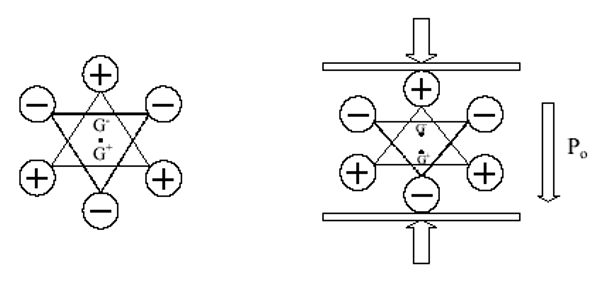
\includegraphics[scale=1]{images/photo21.PNG}
    \end{center}
    
    Mettent en jeu des composants piézoélectrique qui ont la propriété de se polariser électriquement lorsqu'ils sont déformés. Une métallisation des faces permet de recueillir la charge électrique pour en permettre la transformation et l’amplification en tension vers la chaîne de mesure. 
    
\end{itemize}

\subsubsection{Géophone}

Permet de mesurer des ondes sismiques de surface. Il s'agit d'un aimant permanent qui se déplace dans une bobine en même rythme que l'onde sismique et produit ainsi un courant électrique au sein du conducteur bobiné. On mesure la différence de tension aux bornes de cette inductance en sortie du système.

\subsubsection{Sismographe}

Un sismographe est constitué d'une masse (inertielle) fixée au bout d’une barre encastrée à sa base. Un amortisseur y est accouplé afin de stabiliser la masse après une secousse et éviter que le sismographe ne continue à osciller après la fin du séisme et récupère sa position de départ pour enregistrer d'autres évènements. La masse, en raison de son inertie, tend à rester en place alors que le bâti de l'appareil, fixé au sol, accompagne les mouvements du séisme. 

\begin{center}
    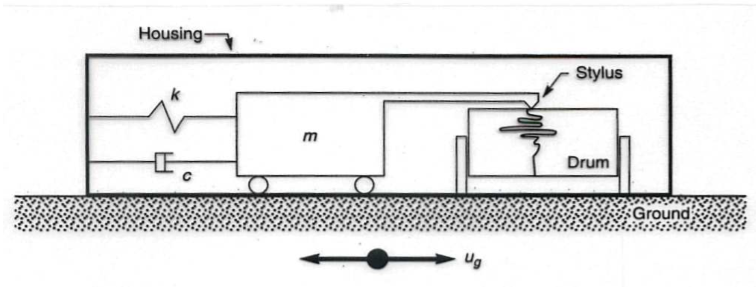
\includegraphics[width=\linewidth]{images/photo22.PNG}
\end{center}

\section{Mécanique des ondes}

Permet de comprendre le comportement d'un pieu sollicité dynamiquement. Permet de déduire la résistance mobilisée par le pieu lors de son enfoncement transitoire.

\subsection{Formule de battage}

\begin{center}
\begin{tabular}{c|c}
$e Q = M g H$
        &  $e$: refus [m] \\
        &  $M$: masse du mouton [kg] \\
        &  $H$: hauteur de chute [m] \\
        &  $Q$: charge [kN] \\
        &  $g$: accélération terrestre [$m/s^2$] 
\end{tabular}
\end{center}

Ce genre de formules considèrent le pieu comme un élément rigide, ce qui est faux. Le choc crée des ondes de compression qui se propagent à une vitesse finie dans le pieu en provoquant un déplacement u(x,t).

\subsubsection{Équation d'onde}

Traduction de la loi de Newton dans un milieu continu : 

\begin{center}
\begin{tabular}{c|c}
$dm = A dx \rho$
        &  $dm$: masse du tronçon \\
        &  $A$: section du pieu \\
        &  $dx$: longueur élémentaire \\
        &  $\rho$: masse volumique 
\end{tabular}
\end{center}

\begin{center}
    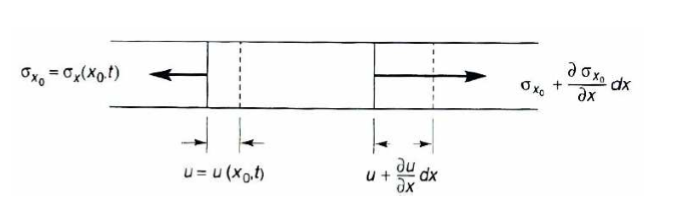
\includegraphics[scale=1]{images/photo23.PNG}
\end{center}

\begin{itemize}
    \item équilibre de translation : 
    $$ dF = A dx \rho \frac{d^2u}{dt^2} $$
    \item contrainte : $\sigma  = \frac{F}{A}$ on peut donc simplifier par $Adx$ 
    $$ \frac{\delta \sigma_x}{\delta x} = \rho \frac{\delta^2 u}{\delta t^2} $$
    \item matériaux élastique : $\sigma = E \frac{du}{dx}$
\end{itemize} 

On obtient l'équation d'onde :

$$\frac{\delta^2 u}{\delta t^2} = \frac{E}{\rho} \frac{\delta^2 u}{\delta x^2}$$

Il s'agit d'une EDP hyperbolique du second ordre qui a pour solution :

$$ u(x,t) = f(\sqrt{\frac{E}{\rho}}.t-x)+g(\sqrt{\frac{E}{\rho}}.t+x) $$

On constate une propagation d'ondes montantes(f) et descendantes(g) dans le pieu. Deux propriétés sont à la source de cette propagation d'ondes : milieu pesant et compressible.

\subsection{Impédance}

\begin{itemize}
    \item Impédance spécifique (ou acoustique) caractérise la résistance d'un milieu au repos à entrer en mouvement. 
    
    \begin{center}
    \begin{tabular}{c|c}
        $I_{\sigma} = \frac{p}{v} = \rho c$
            &  $p$:pression acoustique \\
            &  $v$: vitesse de déplacement local 
    \end{tabular}
    \end{center}
    
    \item Impédance mécanique
    
    \begin{center}
    \begin{tabular}{c|c}
        $I=c_b A \rho$
            &  $A$:section \\
            &  $c_b$: vitesse de déplacement
    \end{tabular}
    \end{center}
\end{itemize}

L’impédance permet donc de relier, en tête de pieu libre, la vitesse à la force exercée. Un pieu semi-infini peut donc être mécaniquement assimilé à un amortisseur de constante $I=\rho cA [MN/ms]$.

\subsection{Calcul de l'impulsion sur un pieu libre semi-infini}

On prend comme hypothèse un pieu élastique semi-infini continu. 

\begin{center}
    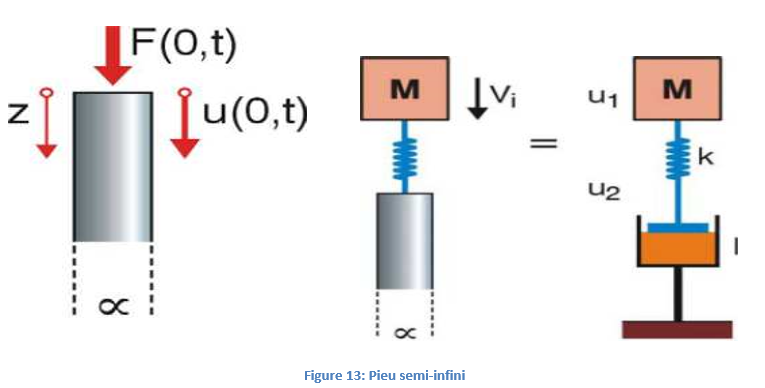
\includegraphics[width=\linewidth]{images/photo24.PNG}
\end{center}

La vitesse d'impact du mouton : 

\begin{center}
\begin{tabular}{c|c}
$v_i = \sqrt{2 \nu g h}$
        &  $\nu$: rendement de la chute \\
        &  $h$: hauteur 
\end{tabular}
\end{center}

 L’art du battage consiste  en effet à enfoncer le pieu sous l’effet du choc sans le casser. Il faut atténuer l'amplitude maximale de l'impulsion en interposant un casque de raideur k. On peu modéliser la tête de pieu comme un système masse-ressort à deux degrés de liberté : u1 (déplacement de la masse) et u2 (déplacement de la tête de pieu). L'équilibre est satisfait pour : 
 
 $$ F = k (u_1 - u_2) = I v_2 = -M \ddot{u}_1 $$
 
 On remarque que l'impédance du pieu et la vitesse d'impact de la masse permettent d'adimensionaliser l'impulsion F(t). Il faudra optimiser la transmission d'énergie : 
 
 $$ E = \int^{\infty}_0 F(t) v(t) dt $$
 
 En gros il faudra bien choisir la masse M et la raideur k en fonction de l'impédance des pieux concernés par le système.
 
 \subsection{Calcul de la réflexion en pointe}
 
 On cherche a calculer analytiquement l'onde générée en tête de pieu soumis à l'impact. L'amortisseur de constante I ne dissipe pas l'énergie, le pieu étant élastique, il restitue intégralement l'énergie qu'il a emmagasinée suite à l'impact. On parle plutôt d'amortissement géométrique (retrouve son calme après le passage de l'onde).
 
 Les pieux étant finis en pratique, il importe d’envisager la génération d’une onde montante en bout de course, c'est-à-dire lorsque l’onde incidente atteint la fin du pieu. 
 
 \begin{itemize}
     \item Si la base du pieu est à l'air libre, son impédance devient brutalement nulle tandis que la condition en cette limite impose une contrainte nulle. Ceci ce traduit par une onde symétrique mais de signe opposée. L'onde descendante de compression rencontre une onde montante de traction dont la superposition entraîne l'annulation de la contrainte.
    $$ F_\text{incidente} = - F_\text{réfléchie} $$
    \item Si il y a une résistance à la base, on superposera une onde de compression montante d'amplitude correspondant au terme de résistance $R_b$ mobilisé à la base à l'onde de traction définie précédemment.
    \item Si il y a une base fixe (résistance infinie), on impose une condition de vitesse nulle à la base. Cette condition se traduit par la coexistence des deux ondes de compression dont la superposition entraîne un doublement de la contrainte à la base.
 \end{itemize}
 
 \subsection{Effet du frottement latéral}
 
 Considérons qu'à une profondeur z*, un terme de frottement latéral $Q_f$ soit mobilisé au passage de l'onde de déplacement. Ce frottement s'oppose au mouvement et être considéré comme la source d'une nouvelle perturbation. Comme le niveau auquel s'exprime cette résistance est interne au domaine, les deux sens de propagation de la perturbation sont matériellement et anti-symétriquement possible. $Q_f$ est repris à part égales entre la partie inférieure et supérieure via création d'une onde de compression montante (frottement positif) et d'une onde de traction descendante (frottement négatif). 
 
 \begin{center}
    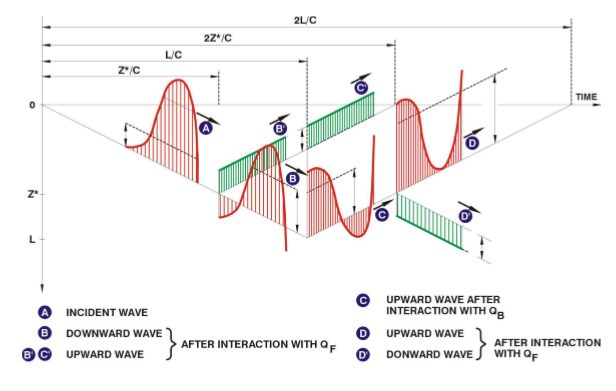
\includegraphics[scale=1]{images/photo25.PNG}
\end{center}

\section{Exploitation des mesures dynamiques}

\subsection{Combinaison d'ondes}

L'identification des efforts résistant repose sur la mesure des amplitudes des ondes incidentes et résistantes. On les déduits des équations d'équilibre d'un élément d'interface pieu-sol. Pour un pieu prismatique d'impédance Z: 

\begin{center}
    \begin{tabular}{c c}
        $F \downarrow = \frac{1}{2}(F+Zv)$ & $F \uparrow = \frac{1}{2}(F-Zv)$ \\
    \end{tabular}
\end{center}

 \begin{center}
    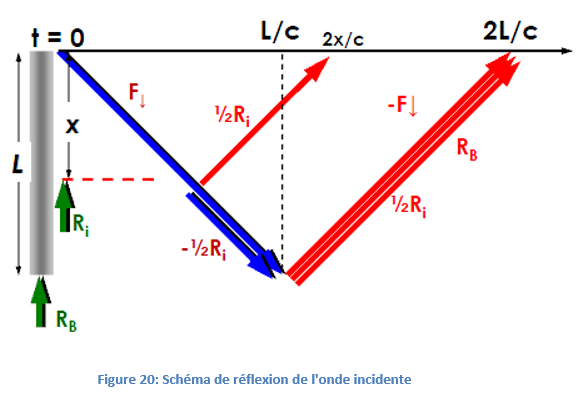
\includegraphics[scale=0.7]{images/photo26.PNG}
\end{center}

La vitesse particulaire de la tête du pieu est proportionnelle à la force descendante.

\begin{center}
    \begin{tabular}{c|c}
        $\frac{\delta ^2u}{\delta t^2}-c^2\frac{\delta^2 u}{\delta x^2} = \frac{R(x,t)}{EA}$ 
            &  R(x,t) résistance mobilisée en x 
    \end{tabular}
\end{center}

\begin{itemize}
    \item Si pieux libre, R(x,t) = 0 on retrouve l'équation d'onde homogène.
    \item Si les réactions de frottement latéral créent des ondes de compression qui remontent en tête de pieu, alors il y a superposition à l'onde de compression, il n'y donc plus proportionnalité entre la vitesse et l'effort normal mesuré. L'onde descendante est réfléchie à la base et reviens avec un écho (=2L/c).
    \item Si on accepte l'hypothèse selon laquelle le frottement latéral et la réaction à la base sont entièrement mobilisés à l'arrivée de l'onde, alors on obtient l'estimation suivante pour la résistance latérale et totale :
    $$ R_lat = F(0,\frac{2l}{c}) - Z.v(0,\frac{2l}{c})$$
    $$ R_lat + R_b = \frac{1}{2}F(0,t*)+F(0,t*+\frac{2l}{c})+Z.v(0,t*)-Z.v(0,t*+\frac{2l}{c}))$$
    avec $\frac{2l}{c}$, le temps nécessaire pour un aller-retour dans le pieu et $t*$, le temps de référence correspondant à l'effort maximum.
\end{itemize}

La vitesse particulaire influence la mobilisation de la résistance à la base et au frottement latéral. La résistance à une composante statique (élasto-plastique) et une composante dynamique (visqueuse) :

 \begin{center}
    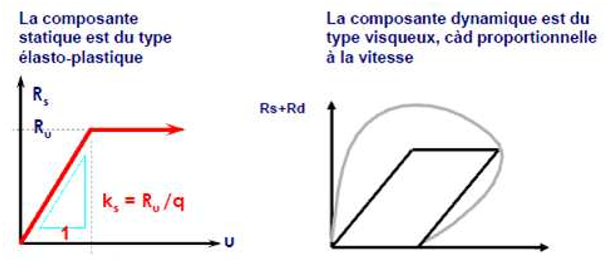
\includegraphics[scale=1]{images/photo27.PNG}
\end{center}

\subsection{Analyse inverse}

La modélisation géotechnique inverse est une démarche d’analyse par laquelle on essaye de déduire les paramètres de comportement du sol au départ de mesures (méthode observationnelle). On dispose de la réponse mesurée du système à une sollicitation connue. Le but est de trouver les paramètres du modèle qui expliqueront aux mieux les observations.

Dans le cas de sollicitations dynamique de pieux, on impose dans le modèle de calcul soit la force, soit la vitesse à la tête du pieu. Imaginons qu'on utilise la vitesse comme condition à la limite supérieur du pieu, on peu alors alors utiliser la force comme signal objectif à reproduire par le calcul. On présume des valeurs de frottement latéral et de résistance à la base et on compare nos réponse calculé. On ajuste nos estimations jusqu'à obtenir une force correspondante.

Une fois que notre modèle correspond, il parait légitime de l'utiliser pour d'autres scénarios de chargement et en particulier celui qui correspond à un essai statique.

On remarque que la vitesse augmente la raideur apparente du pieu, outre l'apport d'une résistance supplémentaire. C'est un effet comparable à celui d'un amortisseur.

\subsection{Etude de la vitesse de chargement}

On utilise l'essai de pénétration à la barre (T-bar). Il est utilisé dans des argiles très molles. Il s'agit d'un pénétromètre avec une pointe remplacée par un cylindre horizontal. Cette forme permet une cinématique de type écoulement sans décollement du sol argileux et non pas un refoulement. L'effort mesuré en pointe peut ainsi être directement relié aux propriétés de résistance du sol. Il permet une reconnaissance de la cohésion non drainée dans les sols mous (contrairement au scissomètre qui ne donne que des profils discrets).

Évaluation de la résistance non drainée au cisaillement : 

\begin{center}
\begin{tabular}{c|c}
$s_u = \frac{P}{d L N_b}$
        &  $P$: effort mesuré \\
        &  $d$: diamètre \\
        &  $L$: longueur \\
        &  $N_b$: facteur adimensionnel [9-12] 
\end{tabular}
\end{center}

Le dispositif permet de mesurer des efforts jusqu'à 375 N en traction ou compression. L'enfoncement est suivi par un potentiomètre rotatif: la profondeur de reconnaissance atteint 400 mm.

Le T-bar permet également d'apprécier la dégradation du massif sol sous l'effet des cycles puisque l'essai peut être réalisé à l'enfoncement, puis complété en remontant le dispositif et en y associant, à une cote précise un certain nombre de cycles.

La résistance est minimale pour une vitesse de pénétration intermédiaire. Elle augmente lorsque la vitesse de pénétration est suffisamment lente pour permettre au sol de s'améliorer par consolidation? Pour des vitesses importantes, un effet de viscosité non linéaire induit une augmentation de la résistance non drainée du sol.

\end{document}
